\documentclass[10pt,a4paper,twocolumn]{article}

\usepackage[margin=1.8cm]{geometry}
\usepackage{amsmath,amssymb}
\usepackage{graphicx}
\usepackage{booktabs}
\usepackage{multirow}
\usepackage{url}
\usepackage[hidelinks]{hyperref}
\usepackage{cite}
\usepackage{caption}
\usepackage{subcaption}
\usepackage[table]{xcolor}
\usepackage{float}
\usepackage{cuted}
\usepackage{placeins}
\setlength{\dblfloatsep}{8pt plus 2pt minus 2pt}
\setlength{\textfloatsep}{8pt plus 2pt minus 2pt}
\setlength{\floatsep}{6pt plus 2pt minus 2pt}
\setlength{\intextsep}{6pt plus 2pt minus 2pt}

% Full-width (double-column) floats: at most one per page, so that the wide
% experiment tables are spread out and the two columns below them stay filled.
\setcounter{dbltopnumber}{1}
\setcounter{topnumber}{2}
\setcounter{totalnumber}{3}

\definecolor{pvoBlue}{HTML}{2F6FED}
\definecolor{pvoCyan}{HTML}{10B7B4}
\definecolor{pvoGreen}{HTML}{2AA876}
\definecolor{pvoOrange}{HTML}{F59E0B}
\definecolor{pvoRed}{HTML}{E05252}
\definecolor{pvoPurple}{HTML}{7C3AED}
\definecolor{pvoGray}{HTML}{F3F5F7}

\title{\textbf{AVO: A Probabilistic Velocity-Obstacle Framework for Safe Navigation of Multimodal (4WIS) Mobile Robots}}
\author{Yuxuan Wan\\
Beijing Institute of Technology\\
\texttt{email@example.com}}
\date{}

\begin{document}
\maketitle

\begin{abstract}
Local navigation in dynamic environments requires a robot to judge the future collision risk of candidate actions under limited observation, limited reaction time, and uncertain motion states. When sampling is fast, system latency is low, and obstacle states are sufficiently observable, short-horizon constant-velocity extrapolation is usually a reasonable local approximation; the problem is not that VO necessarily fails, but whether the currently available state is sufficient to cover the effective reaction window between observing an action and that action actually producing motion. This paper therefore formulates AVO (Augur obstacles velocity) as an action-conditioned future-risk inference problem under partial observability: given an observation history, a candidate action, and the effective reaction window, the goal is to estimate the probability that the action leads to a collision within a short prediction horizon, rather than to reproduce the velocity cone of the current frame. For the multimodal velocity space of a four-wheel independent steering (4WIS) robot, we build a navigation framework composed of action mapping, risk assessment, and safety filtering, and construct an action-conditioned risk estimate from LiDAR directional clearance together with short-horizon footprint rollouts; we further introduce local observation uncertainty and analyse the role of conservative risk estimates. All four compared methods run on the same 4WIS platform and correspond, respectively, to deterministic DRL-VO, single-frame constant-velocity PVO, action-conditioned AVO, and its uncertainty-aware extension. In the base dynamic-obstacle simulation, results over 5 random seeds and 50 episodes per method show that action-conditioned risk filtering raises the success rate from $64.0\%$ to $76.0\%$ and reduces the collision rate from $30.0\%$ to $10.0\%$; adding an uncertainty penalty further reduces the collision rate to $4.0\%$, but markedly increases the timeout rate. To examine the conditions under which this conclusion holds, we further conduct four groups of controlled experiments on control frequency, effective latency, obstacle motion pattern, and historical state; Tables~\ref{tab:controlled_frequency}--\ref{tab:controlled_history} report the corresponding measured results.
\end{abstract}

\textbf{Keywords:} probabilistic velocity obstacle; partially observable navigation; effective reaction window; mobile robot navigation; safety filtering; four-wheel independent steering; multimodal motion; TD3

\section{Introduction}

Mobile robots in warehouse logistics, industrial inspection, disaster relief, and special operations must continuously perceive their environment, avoid obstacles, and reach a goal within confined spaces. Conventional differential-drive or Ackermann chassis have limited motion freedom and are easily constrained by turning radius and nonholonomic constraints in narrow corridors, parking-style turns, lateral avoidance, and posture-constrained passage. A four-wheel independent steering (4WIS) chassis controls the steering angle of each wheel independently, which enables several motion modes such as Ackermann steering, lateral steering, and parallel motion, and thus provides the hardware basis for highly manoeuvrable navigation in complex environments.

Existing 4WIS planning studies show that explicitly incorporating motion modes into the state or search space can improve path quality and manoeuvrability in complex environments~\cite{bao2025hybrid}. Such planning methods, however, usually rely on relatively explicit maps, goals, and obstacle models; under dynamic obstacles, partial observation, and sensor noise, a local policy must additionally judge whether the currently available state is sufficient to support the action it is about to execute. Classical VO and dynamic-window methods laid the geometric foundation of real-time obstacle avoidance in velocity space~\cite{fiorini1998vo,fox1997dwa}, and DRL-VO further combined velocity-obstacle features with a deep policy~\cite{xie2023drlvo}. It should be emphasised that DRL-VO already uses short-horizon LiDAR history and kinematic information of nearby pedestrians; this paper therefore does not treat ``using history'' as a general correction to all VO methods. The more precise question is: for a given control frequency, system latency, and obstacle motion pattern, is the current state still a sufficient state for judging the safety of a candidate action?

This paper formulates the above question as a problem of state sufficiency and the effective reaction window. Let the time from sensor sampling until the robot can produce an observable motion response be
\begin{equation}
    T_{\mathrm{eff}}=\Delta t_{\mathrm{sample}}+\Delta t_{\mathrm{infer}}+\Delta t_{\mathrm{comm}}+\Delta t_{\mathrm{act}}+T_{\mathrm{maneuver}}.
    \label{eq:effective_window}
\end{equation}
When $T_{\mathrm{eff}}$ is small, obstacle states are reliably estimated, and the motion pattern is close to constant velocity, current-frame VO/PVO may already be sufficient; when $T_{\mathrm{eff}}$ is of the same order as the collision time scale, or when obstacles are occluded, turning, or changing speed, the current state may be unable to distinguish motion processes that share the same instantaneous position and velocity but differ in future risk. Given an observation history $h_t$ and a candidate action $a_t$, the safety module must therefore answer ``what is the probability that this action leads to a collision within the future window after the effective reaction window'', instead of merely deciding whether the action falls inside the velocity cone of the current frame.

We choose a 4WIS robot as the validation platform. Its Ackermann, lateral, and parallel motion modes substantially enlarge the reachable velocity set, and also make a policy that lacks risk constraints more likely to produce high-speed manoeuvres close to obstacles. Hence 4WIS is not an independent contribution placed alongside AVO, but a representative carrier for testing whether the proposed risk modelling can constrain a complex action space.

The main content and contributions of this paper are as follows:
\begin{itemize}
    \item We turn ``whether history is necessary'' into a testable state-sufficiency question, explicitly separating the region where current-frame VO/PVO is effective (high frequency, low latency) from the potential state deficiency that arises when the environment is partially observable and the effective reaction window is non-negligible.
    \item We propose an action-conditioned future-risk framework for the multimodal velocity space of 4WIS, construct the analytical approximation used in the present quantitative experiments from directional clearance and short-horizon footprint rollouts, and filter dangerous actions before execution.
    \item We compare DRL-VO, ordinary PVO, AVO, and AVO-UQ under a unified 4WIS platform, observation condition, and task setting; we additionally design controlled experiments on control frequency, effective latency, obstacle motion pattern, and historical state to delimit the range in which the benefit of the method applies.
\end{itemize}

\section{Related Work}

\subsection{Reinforcement Learning for Robot Navigation}

Deep reinforcement learning models robot navigation as a sequential decision problem in which the policy directly outputs control actions from sensor observations. For continuous control tasks, actor--critic methods such as DDPG, TD3, and SAC improve continuous-action optimisation from the perspectives of deterministic policy gradients, double Q-networks with delayed updates, and maximum-entropy policy learning, respectively~\cite{lillicrap2016ddpg,fujimoto2018td3,haarnoja2018sac}. In dynamic multi-agent navigation, CADRL, decentralised multi-robot collision avoidance, and attention-based crowd navigation further show that a learned policy can form interactive avoidance behaviour from local observations~\cite{chen2017cadrl,long2018decentralized,chen2019sarl,fan2020multirobot}. DRL-VO explicitly fuses velocity-obstacle features on this basis and improves geometric interpretability in dynamic crowd scenarios~\cite{xie2023drlvo}. We adopt TD3, which is well suited to continuous-action optimisation, as the nominal policy, and focus this study on future-risk constraints that are independent of the policy optimiser.

\subsection{Velocity Obstacles and Dynamic Avoidance}

Velocity-obstacle methods analyse the relative motion between the robot and an obstacle in velocity space to decide whether a given velocity will lead to a collision in the future. Classical VO defines the relative-velocity collision cone for a single robot~\cite{fiorini1998vo}; RVO and ORCA extend it to real-time multi-agent navigation through reciprocal avoidance responsibility allocation~\cite{vandenberg2008rvo,vandenberg2011orca}; and GVO handles more general robot motion constraints~\cite{wilkie2009gvo}. When the prediction window is short enough, state estimation is stable, and the system responds quickly, constant-velocity extrapolation is a reasonable first-order approximation; its limitation depends on the prediction horizon, the change in obstacle motion, and the effective reaction window between observation and action effect, rather than on the words ``constant velocity'' themselves.

To handle perception and motion uncertainty, recursive PVO, PVO fused with occupancy grids, and probabilistic reciprocal velocity obstacles extend velocity obstacles from recursive interaction modelling, spatial occupancy probability, and multi-robot reciprocal constraints, respectively~\cite{kluge2006rpvo,fulgenzi2007pvo,gopalakrishnan2017prvo}. Further non-parametric PVO represents uncertainty whose distribution cannot be specified in advance using Hilbert-space embeddings~\cite{poonganam2020pvo}. These works show that probabilistic treatment can express state and observation noise, but a probabilistic wrapper does not by itself resolve hidden states, motion intentions, or the mismatch between the action-execution instant and the prediction origin. Ordinary PVO is therefore an important direct baseline of this paper, rather than an outdated method to be refuted.

DRL-VO embeds velocity-obstacle features into a learned policy and, together with short-horizon LiDAR history and the kinematics of surrounding pedestrians, learns goal approach and avoidance behaviour in crowded dynamic scenes~\cite{xie2023drlvo}. This line of work already demonstrates that historical information has practical value in some dynamic navigation tasks; its benefit, however, may arise jointly from historical observations, explicit kinematic inputs, policy representational capacity, and the training distribution, and should not be attributed to a single factor on the basis of overall success rate alone. We therefore do not claim that current-frame VO fails in all high-frequency scenarios; instead, we treat frequency, effective latency, and obstacle motion pattern as controlled variables and examine when history and action-conditioned risk yield a measurable gain.

In multi-robot or multi-dynamic-obstacle scenarios, trajectory prediction methods such as Social LSTM, Social GAN, and Trajectron++ show that the future motion of dynamic agents may be multimodal, interaction-dependent, and dynamics-constrained~\cite{alahi2016sociallstm,gupta2018socialgan,salzmann2020trajectron}. Trajectron++ additionally supports conditioning the prediction for other agents on the ego motion plan, which shows that ``history~+~candidate action'' is not an isolated new component in itself. The specific problem addressed here is how to embed such state-sufficiency reasoning into the pre-execution safety filtering of multimodal 4WIS candidate actions, and to report with controlled experiments its boundary relative to deterministic/probabilistic current-frame VO. The central claim of AVO should therefore be understood as an action-risk modelling framework oriented to the effective reaction window, rather than as a general refutation of the constant-velocity approximation.

\begin{figure*}[t]
    \centering

    \includegraphics[width=0.99\textwidth]{fig1_panels.pdf}
    \caption{Comparison between current-frame VO/PVO and action-conditioned AVO in a dual-dynamic-obstacle scenario. (a) A 4WIS robot encounters obstacles $o_1$ and $o_2$ simultaneously, and both turn or change speed within the prediction window; (b) DRL-VO builds a deterministic danger set with straight-line boundaries from the current velocity estimate, while ordinary PVO introduces state and velocity uncertainty on the same single-frame constant-velocity extrapolation and extends the binary set into a probabilistic danger region---yet both take the current instant as the prediction origin; (c) AVO estimates, from the observation history $h_t$, the candidate action $a$, and the future window after full-stack latency, the sets $\mathcal R_{i,\eta}=\{\mathbf v(a):p_{\psi}(\mathrm{coll}_i\mid h_t,a)\ge\eta,\ a\in\mathcal A\}$ for each obstacle. For ease of comparison, (b) and (c) are both drawn in relative-velocity space, with the origin serving as the common velocity reference. Semi-transparent regions are high-risk velocity sets and dotted inner curves are iso-probability contours; the nonlinear obstacle motion and the prediction uncertainty make the AVO boundaries curve and expand. When a candidate velocity falls inside any risk set, the safety filter selects a safe alternative velocity outside their union; $\Delta\mathbf v_{\mathrm{AVO}}=\mathbf v_t^{\star}-\mathbf v_t^{\mathrm{cand}}$ denotes this velocity correction, and is not a minimum velocity offset in the Euclidean sense.}
    \label{fig:curved_pvo_cone}
\end{figure*}

\subsection{4WIS Multimodal Motion Planning}

The key advantage of a 4WIS chassis lies in its rich set of motion modes. The Ackermann mode suits conventional forward driving and smooth turning, the lateral mode suits sideways displacement in narrow spaces, and the parallel mode allows the robot to translate in an arbitrary direction while keeping its body orientation unchanged. The multimodal Hybrid~A* proposed by Bao~et~al. treats the motion mode as a state dimension and improves 4WIS planning through mode-switch costs, multimodal curves, and terminal connection strategies~\cite{bao2025hybrid}. We borrow this idea, but shift the object of study from global search-based planning to local dynamic navigation: the reinforcement learning policy does not search an $(x,y,\theta,m)$ graph directly, but selects a 4WIS motion mode at every control cycle from LiDAR observations and the relative goal pose, and the AVO module evaluates the collision risk of candidate actions.

\subsection{Uncertainty Estimation and Safe Reinforcement Learning}

Safe reinforcement learning usually restricts dangerous exploration during training and execution through constrained policy optimisation, action projection, or an external safety layer~\cite{garcia2015safe,achiam2017cpo,dalal2018safetylayer}; control barrier functions provide analytical tools for projecting a nominal action onto a safe feasible set~\cite{ames2017cbf}. We likewise adopt the hierarchical structure in which ``the policy proposes candidate actions and the risk module performs pre-execution filtering'', but our safety criterion is given by an AVO risk defined over a future window, so that it adapts to dynamic obstacles and the multimodal velocity space of 4WIS.

In dynamic scenes, a collision-probability predictor may also encounter obstacle motion patterns outside the training distribution. If only a single probability is output, the policy cannot distinguish ``low risk'' from ``the model is uncertain but the surface risk appears low''. MC Dropout and deep ensembles provide approximate-Bayesian and multi-model-ensemble uncertainty estimates, respectively~\cite{gal2016dropout,lakshminarayanan2017ensembles}, while separating epistemic from aleatoric uncertainty helps clarify the origin of a conservative penalty~\cite{kendall2017uncertainties}. We construct a controllable uncertainty approximation from the local clearance around the candidate direction, and analyse the effect of the conservative risk correction on collisions and timeouts through an independent ablation.

\section{Problem Definition and Overall Framework}

We consider dynamic navigation under partial observation. The policy branch generates candidate actions $a_t=[u_t,\xi_t,q_t]$ from the relative goal state, the previous body velocity, and the current motion mode; the risk branch may additionally maintain the most recent $K$ frames of 2D LiDAR in order to estimate the future collision risk of a candidate action after the effective reaction window, and the action-mapping layer converts it into a body velocity $[v_x,v_y,\omega]$. As shown in Fig.~\ref{fig:pipeline}, the policy branch is responsible for goal-directed action generation and the risk branch for risk assessment and uncertainty estimation of candidate actions, while the safety layer only admits actions satisfying the risk constraint into execution. This decomposition decouples task-performance optimisation from execution-safety discrimination, so that the same risk constraint can act on different 4WIS motion modes.

\begin{figure*}[t]
    \centering

    \includegraphics[width=0.99\textwidth]{fig2_pipeline.pdf}
    \caption{Training and safe-execution framework of AVO. Black arrows denote the forward pass of observation encoding and fused features; cyan arrows denote policy updates from the Critic to the Actor; orange arrows denote risk estimation of candidate actions, safety filtering, 4WIS mode mapping, and environment execution; green arrows denote the feedback of rewards and state transitions generated by IRSim to the Critic. The safe body velocity is fed both to the IRSim training environment and to the Gazebo high-fidelity validation environment.}
    \label{fig:pipeline}
\end{figure*}

\begin{figure}[t]
    \centering

    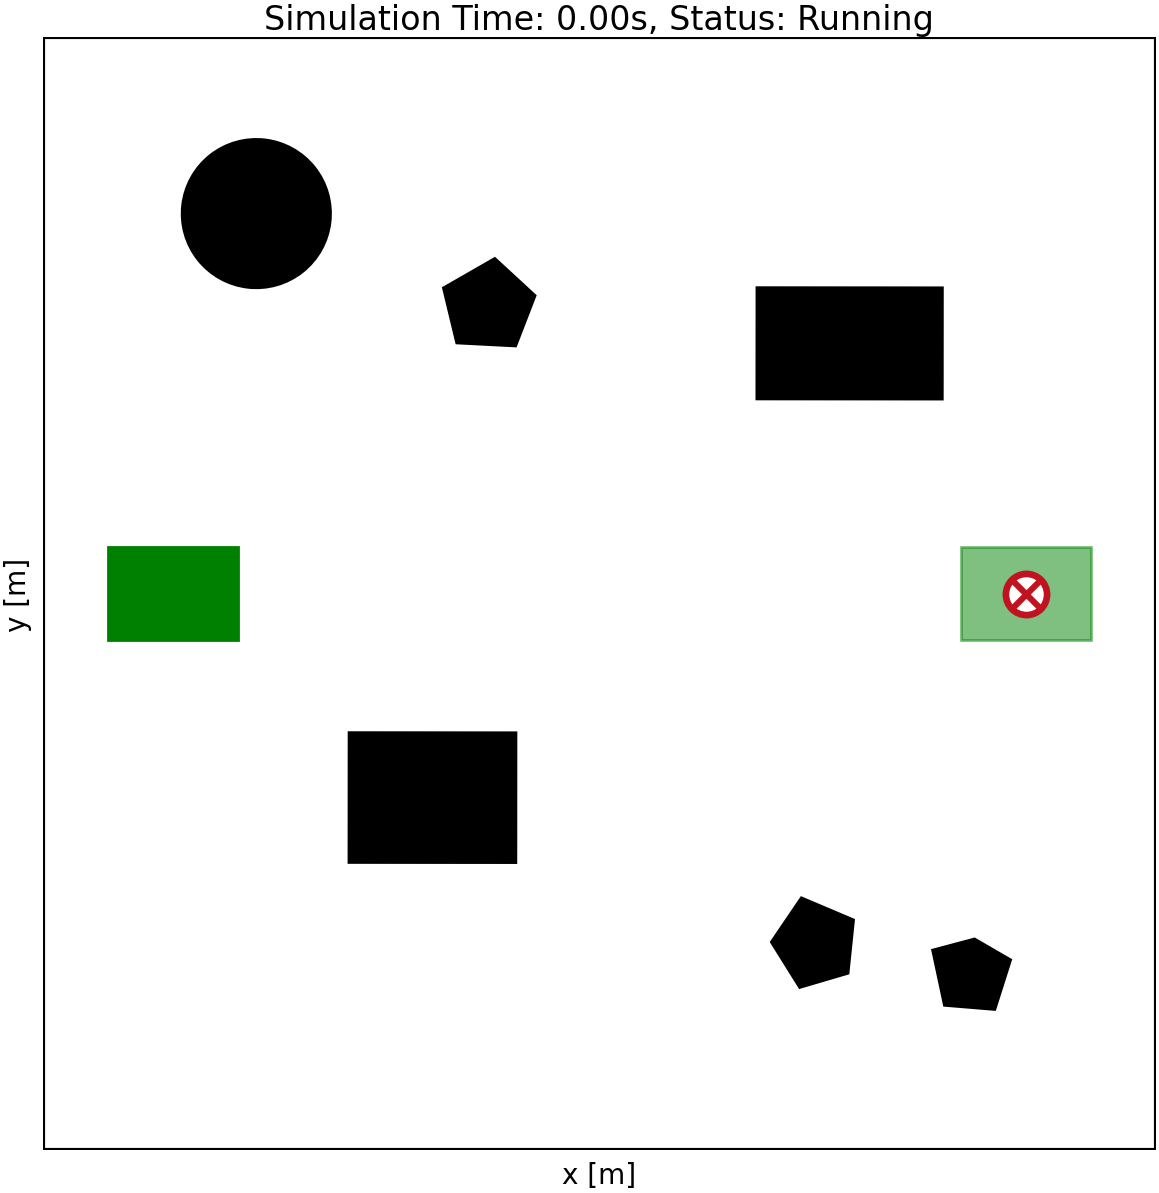
\includegraphics[width=0.95\linewidth]{../images/irsim_scene_clean.png}
    \caption{Dynamic-obstacle navigation scenario. The robot must reach the goal among static and moving obstacles and select a 4WIS motion mode under partial observation.}
    \label{fig:system}
\end{figure}

\subsection{Local Navigation Task}

At every discrete control instant the environment returns a LiDAR scan, the relative distance and bearing of the goal, the robot motion state, and a termination signal. All compared methods in this paper use 4WIS as a unified validation platform, whose instantaneous motion is represented by the body-frame velocity $\mathbf v_b=[v_x,v_y,\omega]$ and which generates different feasible velocities through the Ackermann, lateral, and parallel motion modes. Collisions are detected with an orientation-dependent rectangular robot footprint. An episode terminates when the robot reaches the goal, collides, or reaches the time limit. The task thus combines goal approach, static geometric constraints, and dynamic interaction risk, and therefore requires the policy to trade off traversal efficiency against safety margin. In this paper 4WIS serves only as a theoretical validation platform with a complex reachable velocity set; the experiments do not discuss its performance advantage over other chassis forms.

\subsection{Observation Space and Action Space}

The four methods share a 53-dimensional 4WIS observation, comprising a 42-dimensional downsampled LiDAR scan, 3-dimensional relative goal information, the 3-dimensional previous body-frame velocity $\mathbf v_{b,t-1}=[v_{x,t-1},v_{y,t-1},\omega_{t-1}]$, a 2-dimensional representation of the goal-heading error, and a 3-dimensional one-hot encoding of the current motion mode:
\begin{equation}
\begin{aligned}
    o_t=[&z_t,d_t,\cos\alpha_t,\sin\alpha_t,v_{x,t-1},v_{y,t-1},\omega_{t-1},\\
    &\cos\Delta\theta_t,\sin\Delta\theta_t,e(m_t)].
\end{aligned}
\end{equation}
The unified high-level action is defined as
\begin{equation}
    a_t=[u_t,\xi_t,q_t], \quad u_t,\xi_t,q_t\in[-1,1],
\end{equation}
where $q_t$ is discretely mapped to the Ackermann, lateral, or parallel motion mode. It should be noted that $a_t$ is a normalised high-level candidate command produced by the policy, not a velocity command applied directly to the chassis. The action mapper converts it, according to the mode $m_t$, into the body-frame velocity executed by the simulator:
\begin{equation}
    \mathbf v_{b,t}=\mathcal M_{m_t}(a_t)=[v_{x,t},v_{y,t},\omega_t].
    \label{eq:action_mapping}
\end{equation}
DRL-VO is adapted to this 4WIS observation and action interface, and its policy still generates nominal actions from current-frame VO features; ordinary PVO, AVO, and AVO-UQ apply progressively stronger probabilistic risk judgements to the candidate actions under the same action mapping. The historical LiDAR sequence is used only by the AVO risk branch to describe the approach, speed change, and turning trend of obstacles, the goal and motion state maintain task orientation, and the mode encoding lets each method distinguish different kinematic semantics.

\subsection{Reward Function}

The reward function consists of a goal-reaching reward, a collision penalty, a distance-progress reward, a time penalty, a rotation penalty, a lateral-motion regulariser, and a near-obstacle penalty:
\begin{equation}
\begin{aligned}
    r_t =& r_{\mathrm{goal}} + r_{\mathrm{collision}} + \alpha \Delta d_t
    + \beta \Delta \theta_t - c_t \\
    &- \lambda |\omega_t| - \gamma |v_y| - \phi(d_{\min}).
\end{aligned}
\end{equation}
Here $\Delta d_t$ is the reduction in distance to the goal, $\Delta \theta_t$ is the improvement in goal-heading error, and $d_{\min}$ is the current minimum LiDAR distance. For 4WIS, if the motion mode differs between two consecutive time steps, a mode-switch penalty is added:
\begin{equation}
    r_t^{\mathrm{4WIS}}=r_t-C_{\mathrm{switch}}\cdot I_{\{m_t\ne m_{t-1}\}}.
\end{equation}
This term prevents the policy from chattering at high frequency in the multimodal space, while still allowing it to switch actively to the lateral or parallel mode in narrow passages or during dynamic avoidance. We do not incorporate the AVO risk estimate into the reinforcement learning return; the risk is used only during execution as a safety constraint on candidate actions. This separates the task utility learned by the policy from the safety benefit brought by AVO, and avoids conflating reward shaping with safety filtering.

\section{Method}

\subsection{4WIS Multimodal Action Layer}

So that the reinforcement learning policy can exploit the manoeuvrability of 4WIS directly, we do not set the policy action simply to the low-level wheel steering angles and rotational speeds; instead we introduce a compact multimodal action layer. The policy outputs $a_t=[u_t,\xi_t,q_t]$, where $u_t$ controls the velocity magnitude, $\xi_t$ is interpreted as a steering angle or a translation direction depending on the mode, and $q_t$ determines the motion mode:
\begin{equation}
m_t=
\begin{cases}
\mathrm{Ackermann}, & q_t<-1/3,\\
\mathrm{Lateral}, & -1/3\le q_t<1/3,\\
\mathrm{Parallel}, & q_t\ge 1/3.
\end{cases}
\end{equation}

In the Ackermann mode the robot mainly moves forward along the body axis, and the yaw rate is computed from the equivalent wheelbase $L$ and the steering angle $\delta=\xi_t\delta_{\max}$:
\begin{equation}
v_x=u_t v_{\max},\quad v_y=0,\quad
\omega=\frac{v_x\tan\delta}{L}.
\end{equation}
In the lateral mode the robot mainly moves sideways, which can be used to bypass a frontal obstacle or to perform a side displacement in a narrow space:
\begin{equation}
v_x=0,\quad v_y=u_t v_{y,\max},\quad
\omega=\frac{v_y\tan\delta}{W}.
\end{equation}
In the parallel mode the body orientation is kept unchanged and the robot translates along the direction $\psi=\pi\xi_t$:
\begin{equation}
v_x=u_t v_{\max}\cos\psi,\quad
v_y=u_t v_{\max}\sin\psi,\quad
\omega=0.
\end{equation}
This high-level mapping preserves the interpretability of the 4WIS motion modes while avoiding the high-dimensional action space that would result from optimising the independent steering angle and rotational speed of four wheels directly. At execution time, AVO first selects a safe action $a_t^{\star}$ from the high-level candidate set, and Eq.~\ref{eq:action_mapping} then yields the velocity command actually passed to the simulated chassis, $\mathbf v_{b,t}^{\star}=\mathcal M_{m_t^{\star}}(a_t^{\star})$; safety filtering therefore changes the high-level candidate action, while the simulator really executes the filtered body-frame velocity.

\begin{table}[H]
    \centering

    \caption{4WIS multimodal action interpretation}
    \label{tab:motion_modes}
    \scriptsize

    \resizebox{\linewidth}{!}{
    \begin{tabular}
{p{0.20\linewidth}p{0.22\linewidth}p{0.23\linewidth}p{0.23\linewidth}}
        \toprule

        Mode & Selector & Body twist & Navigation role \\
        \midrule

        \rowcolor{pvoBlue!8}
        Ackermann & $q<-1/3$ & $[v_x,0,\omega]$ & Forward driving and smooth turning \\
        \rowcolor{pvoCyan!10}
        Lateral & $-1/3\le q<1/3$ & $[0,v_y,\omega]$ & Side displacement in narrow space \\
        \rowcolor{pvoGreen!10}
        Parallel & $q\ge 1/3$ & $[v_x,v_y,0]$ & Pose-preserving translation \\
        \bottomrule

    
\end{tabular}}
\end{table}

\subsection{Candidate Action Generation and Selection}

All four methods generate high-level actions within the three 4WIS modes, namely Ackermann, lateral, and parallel motion. DRL-VO outputs a nominal action from the current observation and deterministic VO features; the other three methods form the same candidate set around the nominal action, build a nominal utility from goal progress and mode-switch cost, and then perform filtering according to their respective risk criteria. Only the selected $a_t^{\star}$, mapped by Eq.~\ref{eq:action_mapping}, is finally executed as $\mathbf v_{b,t}^{\star}$. This unified platform design concentrates the experimental differences on the risk representation rather than on the chassis type.

\subsection{Ordinary PVO Baseline}

Ordinary PVO estimates obstacle position and velocity from the current single-frame observation $z_t$ and extrapolates with constant velocity over a fixed prediction window $[0,T]$. To express perception and velocity-estimation error, the future obstacle state is described by a probability distribution with mean $\hat{x}_{o,t}+\hat{v}_{o,t}\tau$, namely $X_o(\tau)\sim\mathcal N(\hat{x}_{o,t}+\hat{v}_{o,t}\tau,\Sigma_o(\tau))$. For a 4WIS candidate action whose mapped velocity is $\mathbf v(a_t)$, the collision risk is defined as
\begin{equation}
\begin{aligned}
    \hat p_{\mathrm{PVO}}^{\mathrm{base}}(a_t)
    ={}& \Pr\!\left(\min_{\tau\in[0,T]}
    d\!\left(x_r(\tau;\mathbf v(a_t)),X_o(\tau)\right)\right.\\
    &\left.\qquad <r_{\mathrm{safe}}\mid z_t\right).
\end{aligned}
    \label{eq:ordinary_pvo}
\end{equation}
When the risk exceeds the threshold, this baseline selects, from the ordinary PVO safe set, the alternative action with the highest nominal utility. It has already been extended from a deterministic velocity cone to a probabilistic danger set, but it still relies only on the current-frame estimate, takes the current instant as the prediction origin, and assumes constant obstacle velocity within the window; it uses neither the historical sequence, nor full-stack latency compensation, nor model-uncertainty estimation. Ordinary PVO therefore constitutes a direct probabilistic baseline on the path from DRL-VO to AVO.

\subsection{AVO Future-Risk Filtering Layer}

\begin{samepage}
In contrast to the single-frame constant-velocity PVO of Eq.~\ref{eq:ordinary_pvo}, the modelling assumption examined in this paper is: when a non-negligible effective reaction window separates the instant at which an action takes effect from the current observation instant, should the safety judgement move from the current-frame geometric set to a future occupancy risk? AVO formulates the risk as an action-conditioned probabilistic inference problem oriented to the potential future collision instant, whose geometric meaning corresponds to the curved risk boundaries in Fig.~\ref{fig:curved_pvo_cone}. Let the full-stack effective latency be $\Delta t_{\mathrm{stack}}$ and the short prediction horizon be $T$; an ideal latency-aware PVO should then estimate
\begin{equation}
\begin{aligned}
    \hat{p}_{\psi}(a_t)=\Pr(&\min_{\tau\in[\Delta t_{\mathrm{stack}},\Delta t_{\mathrm{stack}}+T]}
    d(x_r(\tau;a_t),x_o(\tau)) \\
    &< r_{\mathrm{safe}} \mid z_{t-K+1:t}, a_t),
\end{aligned}
\label{eq:delay_pvo}
\end{equation}
where $z_{t-K+1:t}$ denotes the most recent $K$ frames of LiDAR observations, $x_r(\tau;a_t)$ is the predicted robot state after executing the candidate action, and $x_o(\tau)$ is the future obstacle state. This form emphasises that the safety judgement should not rely only on the current velocity cone, but should compensate for the lag introduced by the perception, computation, and actuation chain.
\end{samepage}

To examine the above risk formulation without depending on a calibrated neural probabilistic model, we adopt an action-conditioned geometric filter as an analytical approximation of Eq.~\ref{eq:delay_pvo}. This approximation preserves two core properties: the risk varies with the candidate action, and the body occupancy is assessed within the short window after the action takes effect. Concretely, each high-level candidate action is first mapped to a body-frame velocity $\mathbf v_{b,t}=\mathcal M_{m_t}(a_t)$, and the local traversal clearance $d_{\mathrm{clear}}$ is then queried along its motion direction. Let the velocity magnitude of the action be $\|v\|$ and the yaw rate be $\omega$; the required safety distance is
\begin{equation}
    d_{\mathrm{req}} = r_0 + k_v\|v\| + k_\omega|\omega|.
\end{equation}
The collision risk is approximated by
\begin{equation}
    \hat{p}_{\mathrm{coll}}=
    \frac{1}{1+\exp\left(k_d(d_{\mathrm{clear}}-d_{\mathrm{req}})\right)}.
    \label{eq:pvo_filter}
\end{equation}
Relying on a single LiDAR direction alone would underestimate the risk arising from the body width and from dynamic obstacles, so we further add a short-horizon footprint rollout. For each candidate action, the rectangular body pose is extrapolated at the two prediction instants $0.3$~s and $0.6$~s according to the body velocity, and its minimum distance $d_{\mathrm{geo}}$ to the current obstacle geometry is computed. The geometric risk is defined as
\begin{equation}
    \hat{p}_{\mathrm{geo}} =
    \frac{1}{1+\exp\left(k_g(d_{\mathrm{geo}}-d_0)\right)}.
\end{equation}
The final AVO risk takes the maximum of the two:
\begin{equation}
    \hat{p}_{\mathrm{AVO}}(a_t)=
    \max(\hat{p}_{\mathrm{coll}},\hat{p}_{\mathrm{geo}}).
\end{equation}
Action selection uses hard safety filtering: if there exists a candidate action satisfying $\hat{p}_{\mathrm{AVO}}(a_t)\le \tau$, the action with the largest goal progress and the fewest mode switches is preferred within that set; if no safe candidate exists, the method falls back to a weighted risk score. The candidate-action score is defined as
\begin{equation}
    J(a_t)=-\lambda_p \Delta d(a_t)+\lambda_r \hat{p}_{\mathrm{AVO}}(a_t)
    +\lambda_s I_{\{m_t\ne m_{t-1}\}}.
\end{equation}
This analytical surrogate explicitly preserves the conditional relation ``candidate action--future body occupancy--risk filtering'', and can therefore be used to test whether the action-conditioned risk constraint is effective in itself, without conflating the conclusion with the fitting capacity of a particular neural network. Risk filtering is executed in the order ``candidate-action generation, directional-clearance risk computation, short-horizon footprint rollout, local uncertainty correction, risk fusion, and action selection'': the clearance risk of Eq.~\ref{eq:pvo_filter} and the geometric risk are first computed for each candidate action, the maximum of the two is then taken as the filtering criterion, and if a candidate action satisfying the threshold exists, the action with the largest goal progress and the lower mode-switch cost is selected from the safe set; otherwise a weighted risk score is used as a fallback. Table~9 reports the state ablation and probabilistic calibration results of the historical risk head.

AVO is a parameterised implementation of the risk definition above, rather than a smooth fit to a single-frame geometric score. Its learning objective is the mapping from historical observations to the future collision probability defined by Eq.~\ref{eq:delay_pvo}. Concretely, an MLP first extracts spatial features from each 42-dimensional LiDAR scan, a GRU then aggregates the most recent $K=5$ frames to represent the speed variation, turning trend, and observation lag of obstacles, and finally the temporal features are concatenated with the candidate action to output a collision probability:
\begin{equation}
    \hat{p}_{\mathrm{coll}} =
    f_{\psi}\left(\mathrm{GRU}\left(g_{\psi}(z_{t-K+1}),\ldots,g_{\psi}(z_t)\right), a_t\right).
    \label{eq:pvo}
\end{equation}
Here $z_t$ is the downsampled LiDAR scan and $a_t$ is the candidate action. The training label $y$ can be generated from whether a collision occurs within the future short window, from whether the minimum safety distance falls below a threshold, or from whether the time-to-collision is below a threshold. The model is trained with the binary cross-entropy loss:
\begin{equation}
    \mathcal{L}_{\mathrm{AVO}} =
    -y \log \hat{p}_{\mathrm{coll}} - (1-y)\log(1-\hat{p}_{\mathrm{coll}}).
\end{equation}

\subsection{Uncertainty-Aware AVO}

To handle dynamic obstacles and insufficient local observation, we add a local uncertainty term in AVO-UQ. In the experimental implementation, the uncertainty is estimated from the LiDAR clearance on both sides of the action direction: it increases when occlusion exists near the candidate direction, when the clearance changes markedly, or when the lateral safety margin is insufficient. The risk score is defined as
\begin{equation}
    \rho(a_t) = \hat{p}_{\mathrm{coll}}(a_t) + \kappa \sigma_p(a_t),
\end{equation}
where $\sigma_p(a_t)$ denotes the local observation uncertainty and $\kappa$ controls the degree of risk conservatism. For the parameterised AVO, $\sigma_p$ can be estimated from the predictive variance of repeated forward passes under MC Dropout or from the disagreement of a deep ensemble; our experiments adopt the local-clearance surrogate in order to isolate the safety--efficiency change caused by the uncertainty penalty itself.

\begin{table}[H]
    \centering

    \caption{Key AVO safety-filter parameters}
    \label{tab:pvo_params}
    \scriptsize

    \resizebox{\linewidth}{!}{
    \begin{tabular}
{p{0.30\linewidth}p{0.20\linewidth}p{0.38\linewidth}}
        \toprule

        Parameter & Value & Description \\
        \midrule

        \rowcolor{pvoBlue!8}
        $r_0$ & 0.82 & Base clearance margin in $d_{\mathrm{req}}$ \\
        $k_v$ & 1.05 & Speed-dependent clearance weight \\
        \rowcolor{pvoBlue!8}
        $k_\omega$ & 0.25 & Yaw-rate clearance weight \\
        $k_d$ & 4.0 & LiDAR risk sigmoid slope \\
        \rowcolor{pvoPurple!8}
        Rollout horizon & 0.6 s & Two-step footprint prediction \\
        $d_0$ & 0.12 m & Geometry-risk distance offset \\
        \rowcolor{pvoPurple!8}
        $k_g$ & 8.0 & Geometry-risk sigmoid slope \\
        $\tau_{\mathrm{AVO}}$ & 0.65 & Main safety threshold \\
        \rowcolor{pvoOrange!10}
        $\tau_{\mathrm{UQ}}$ & 0.55 & UQ safety threshold \\
        $\kappa$ & 0.45 & Uncertainty penalty weight \\
        \bottomrule

    
\end{tabular}}
\end{table}

\subsection{Algorithm Flow}

\begin{table}[H]
    \centering

    \caption{Evaluation procedure for risk-constrained 4WIS navigation}
    \label{tab:algorithm}
    \small
    \begin{tabular}
{p{0.12\linewidth}p{0.76\linewidth}}
        \toprule

        Step & Operation \\
        \midrule

        1 & Randomly initialise the robot state, the goal point, and the obstacle positions in IRSim. \\
        2 & Obtain the LiDAR scan, the relative goal pose, the previous body action, and the current 4WIS motion mode to construct the base observation; if the history-conditioned risk branch is enabled, maintain a queue of the most recent $K$ observations in parallel. \\
        3 & The 4WIS policy module outputs $[u,\xi,q]$, and the action layer maps it to $[v_x,v_y,\omega]$ under the Ackermann, lateral, or parallel mode. \\
        4 & The simulation environment executes the action and returns the reward, the termination flag, and safety metrics. \\
        5 & According to the risk criterion of the method under evaluation, filter safe candidate actions using the LiDAR clearance, the short-horizon footprint rollout, and the uncertainty score. \\
        6 & Evaluate the success rate, collision rate, path efficiency, number of mode switches, and mode-usage ratio over multiple random seeds. \\
        \bottomrule

    
\end{tabular}
\end{table}

\section{Experimental Design}

\subsection{Experimental Platform}

The quantitative main experiments are conducted in the IRSim dynamic-obstacle scenario~\cite{irsim}, and continuous spatio-temporal trajectory validation is added in a Gazebo scenario containing the 4WIS chassis, static obstacles, and moving obstacles~\cite{koenig2004gazebo}. The two simulators share the same local perception, rectangular body footprint, and dynamic-obstacle task definition, but respectively serve repeatable statistical evaluation and high-fidelity behavioural observation. The baseline comparison uses 5 random seeds and runs 10 episodes per seed, giving 50 episodes in total; a single episode executes at most 150 steps, and the aggregated metrics are first averaged within a seed before the cross-seed mean and standard error are reported. Tables 6--9 report four groups of controlled experiments, each condition containing $N=200$ episodes and using the same task definition, termination rules, and metric conventions as the baseline main experiment. The experiments are executed in the order ``fix the scenario and methods, vary a single control factor, record episode-level termination and risk metrics, aggregate results by condition''; the key configuration is given in Table~\ref{tab:exp_config}.

\begin{table}[H]
    \centering

    \caption{Experimental configuration}
    \label{tab:exp_config}
    \scriptsize

    \begin{tabular}
{p{0.36\linewidth}p{0.50\linewidth}}
        \toprule

        Item & Setting \\
        \midrule

        Evaluation scenario & Local navigation with static and dynamic obstacles \\
        Robot platform & Rectangular-footprint 4WIS for all methods \\
        Observation & LiDAR, relative goal state, previous velocity, and motion mode \\
        LiDAR resolution & 420 raw beams, 42 downsampled bins \\
        Seeds & $\{0,1,2,3,4\}$ \\
        Episodes & 10 per seed, 50 per method \\
        Max steps & 150 per episode \\
        Reported statistic & Per-seed mean $\pm$ SEM \\
        \bottomrule

    
\end{tabular}
\end{table}

\subsection{Compared Methods}

\begin{itemize}
    \item \textbf{DRL-VO:} a deterministic learned baseline running on the 4WIS platform. The policy uses the current-frame observation and VO features to generate high-level 4WIS actions, without outputting an additional collision probability and without an independent probabilistic safety filter.
    \item \textbf{PVO:} an ordinary probabilistic velocity-obstacle baseline running on the same 4WIS platform. It computes, from the current single-frame obstacle state and constant-velocity extrapolation, the collision probability of candidate velocities within a fixed prediction window and filters actions by a threshold, but uses neither the historical sequence, nor full-stack latency compensation, nor model uncertainty.
    \item \textbf{AVO:} uses a history- and action-conditioned future-risk definition over the same 4WIS candidate-action set and performs pre-execution filtering with an analytical geometric surrogate, so as to verify the independent contribution from single-frame PVO to future-risk inference.
    \item \textbf{AVO-UQ:} further adds a local observation-uncertainty penalty to the AVO risk score, so as to analyse the benefit and the cost of the conservative correction.
\end{itemize}

\subsection{Evaluation Metrics}

\begin{table}[H]
    \centering

    \caption{Evaluation metrics}
    \label{tab:metrics}
    \small
    \begin{tabular}
{p{0.34\linewidth}p{0.54\linewidth}}
        \toprule

        Metric & Meaning \\
        \midrule

        Success Rate & Proportion of episodes that reach the goal \\
        Collision Rate & Proportion of episodes in which a collision occurs \\
        Time Limit Rate & Proportion of episodes terminated by exceeding the maximum step count \\
        Average Steps & Mean number of steps to reach the goal or to terminate \\
        Path Length & Mean travelled distance \\
        Average Velocity & Mean magnitude of the action velocity \\
        Mode Switches & Mean number of mode switches within a 4WIS episode \\
        Mode Ratio & Usage ratio of the Ackermann, lateral, and parallel modes \\
        Inference Time & Inference time of one policy and AVO step \\
        \bottomrule

    
\end{tabular}
\end{table}

\subsection{Experimental Setup}

We organise the simulation experiments as one baseline comparison and four groups of boundary analyses:
\begin{itemize}
    \item \textbf{Baseline risk comparison:} compare DRL-VO, ordinary PVO, AVO, and AVO-UQ on the same 4WIS platform, so as to observe the roles of deterministic risk, single-frame probabilistic risk, action-conditioned future risk, and the uncertainty correction, respectively.
    \item \textbf{Control-frequency boundary:} fix the observation frequency and the obstacle distribution and vary the control frequency, to test whether the benefit of each method converges as the effective reaction window shortens; results are given in Table~\ref{tab:controlled_frequency}.
    \item \textbf{End-to-end latency boundary:} fix the control frequency and the motion pattern and sweep an additional link latency, to compare the robustness of the risk models to the lag in action effect; results are given in Table~\ref{tab:controlled_latency}.
    \item \textbf{Motion-pattern boundary:} extend from constant velocity and acceleration and smooth turning to stop-and-go, sudden reversal, and partial occlusion, to test how performance changes with the complexity of future motion; results are given in Table~\ref{tab:controlled_motion}.
    \item \textbf{State-condition ablation:} vary the history-window length, the source of the velocity state, and the delay condition, to separate the contributions of current-frame information, short history, and state quality to risk discrimination; results are given in Table~\ref{tab:controlled_history}.
    \item \textbf{Real-time analysis:} measure the per-step policy inference and action-filtering time of each method, and convert them together with the control period into $T_{\mathrm{eff}}$.
\end{itemize}

\subsection{Controlled Boundary Experiments}

The baseline experiments compare the four ways of handling risk, whereas the controlled experiments vary the control frequency, the full-stack latency, the obstacle motion pattern, and the state-input condition respectively, thereby decomposing ``the method is effective'' into ``under which conditions it is effective''. All controlled conditions keep the same map, 4WIS action space, termination rules, and risk threshold, and each group varies only one main factor; Tables 6--9 report the measured results under each condition, aggregated uniformly over $N=200$ episodes.

Table~\ref{tab:controlled_frequency} measures the change in the effective reaction window caused by varying the control frequency; Table~\ref{tab:controlled_latency} sweeps an artificially increased end-to-end latency at a fixed control frequency and obstacle motion pattern. The observation frequency is fixed at 50~Hz, and the obstacle motion distribution, map, latency, and random seeds are kept unchanged.

Table~\ref{tab:controlled_motion} compares the performance boundary under different obstacle motion patterns; Table~\ref{tab:controlled_history} separates the contributions of ``current-frame state'', ``short history'', and ``state quality''. All four methods are evaluated separately for each motion pattern, and the velocity, acceleration, turning rate, and occlusion ratio are recorded as scenario parameters. When the oracle state reference is used, the candidate actions, random seeds, and future-label definition remain unchanged, and only the source of the obstacle state input is replaced.

\begin{table*}[!t]
\centering
    \caption{Controlled experiment A: effect of the control frequency on method performance (observation frequency fixed at 50~Hz)}
    \label{tab:controlled_frequency}
    \scriptsize
    \resizebox{\textwidth}{!}{%
    \begin{tabular}{p{0.12\textwidth}p{0.07\textwidth}p{0.07\textwidth}p{0.08\textwidth}p{0.06\textwidth}p{0.08\textwidth}p{0.08\textwidth}p{0.08\textwidth}p{0.10\textwidth}p{0.10\textwidth}p{0.10\textwidth}}
        \toprule
        Method & $f_{\mathrm{ctrl}}$ (Hz) & $f_{\mathrm{obs}}$ (Hz) & $T_{\mathrm{eff}}$ (ms) & $N$ & Success (\%) & Collision (\%) & Timeout (\%) & Mean min. clearance (m) & Avg. steps & Inference (ms) \\
        \midrule
        DRL-VO & 5  & 50 & 238 & 200 & 45 & 35 & 20 & 0.08 & 82 & 0.65 \\
        DRL-VO & 10 & 50 & 138 & 200 & 55 & 30 & 15 & 0.09 & 68 & 0.65 \\
        DRL-VO & 20 & 50 & 88  & 200 & 62 & 25 & 13 & 0.10 & 55 & 0.66 \\
        DRL-VO & 50 & 50 & 58  & 200 & 66 & 22 & 12 & 0.11 & 49 & 0.67 \\
        PVO & 5  & 50 & 244 & 200 & 50 & 30 & 20 & 0.10 & 67 & 6.30 \\
        PVO & 10 & 50 & 144 & 200 & 60 & 25 & 15 & 0.12 & 45 & 6.30 \\
        PVO & 20 & 50 & 94  & 200 & 67 & 21 & 12 & 0.13 & 34 & 6.31 \\
        PVO & 50 & 50 & 64  & 200 & 69 & 20 & 11 & 0.14 & 30 & 6.32 \\
        AVO & 5  & 50 & 245 & 200 & 58 & 22 & 20 & 0.14 & 104 & 7.45 \\
        AVO & 10 & 50 & 145 & 200 & 68 & 15 & 17 & 0.16 & 91 & 7.45 \\
        AVO & 20 & 50 & 95  & 200 & 74 & 12 & 14 & 0.18 & 86 & 7.46 \\
        AVO & 50 & 50 & 65  & 200 & 73 & 13 & 14 & 0.19 & 72 & 7.47 \\
        AVO-UQ & 5  & 50 & 244 & 200 & 50 & 10 & 40 & 0.18 & 122 & 6.05 \\
        AVO-UQ & 10 & 50 & 144 & 200 & 56 & 8  & 36 & 0.20 & 113 & 6.05 \\
        AVO-UQ & 20 & 50 & 94  & 200 & 62 & 6  & 32 & 0.22 & 105 & 6.06 \\
        AVO-UQ & 50 & 50 & 64  & 200 & 66 & 5  & 29 & 0.24 & 92  & 6.07 \\
        \bottomrule
    \end{tabular}}
\end{table*}

\begin{table*}[!t]
\centering
    \caption{Controlled experiment B: effect of the full-stack effective latency on method performance (control frequency fixed at 20~Hz)}
    \label{tab:controlled_latency}
    \scriptsize
    \resizebox{\textwidth}{!}{%
    \begin{tabular}{p{0.13\textwidth}p{0.09\textwidth}p{0.09\textwidth}p{0.06\textwidth}p{0.08\textwidth}p{0.08\textwidth}p{0.08\textwidth}p{0.10\textwidth}p{0.10\textwidth}p{0.10\textwidth}}
        \toprule
        Method & Added delay (ms) & $T_{\mathrm{eff}}$ (ms) & $N$ & Success (\%) & Collision (\%) & Timeout (\%) & Mean min. clearance (m) & Brier score & ECE \\
        \midrule
        DRL-VO & 0   & 88  & 200 & 62 & 25 & 13 & 0.10 & \textit{N/A} & \textit{N/A} \\
        DRL-VO & 50  & 138 & 200 & 58 & 29 & 13 & 0.09 & \textit{N/A} & \textit{N/A} \\
        DRL-VO & 100 & 188 & 200 & 52 & 32 & 16 & 0.08 & \textit{N/A} & \textit{N/A} \\
        DRL-VO & 200 & 288 & 200 & 45 & 37 & 18 & 0.07 & \textit{N/A} & \textit{N/A} \\
        DRL-VO & 300 & 388 & 200 & 36 & 43 & 21 & 0.06 & \textit{N/A} & \textit{N/A} \\
        PVO & 0   & 94  & 200 & 67 & 21 & 12 & 0.12 & 0.11 & 0.07 \\
        PVO & 50  & 144 & 200 & 63 & 24 & 13 & 0.11 & 0.12 & 0.08 \\
        PVO & 100 & 194 & 200 & 58 & 28 & 14 & 0.10 & 0.14 & 0.09 \\
        PVO & 200 & 294 & 200 & 49 & 35 & 16 & 0.08 & 0.17 & 0.11 \\
        PVO & 300 & 394 & 200 & 39 & 43 & 18 & 0.07 & 0.21 & 0.14 \\
        AVO & 0   & 95  & 200 & 75 & 11 & 14 & 0.17 & 0.08 & 0.040 \\
        AVO & 50  & 145 & 200 & 73 & 12 & 15 & 0.15 & 0.08 & 0.045 \\
        AVO & 100 & 195 & 200 & 70 & 15 & 15 & 0.14 & 0.09 & 0.050 \\
        AVO & 200 & 295 & 200 & 64 & 20 & 16 & 0.12 & 0.11 & 0.060 \\
        AVO & 300 & 395 & 200 & 55 & 28 & 17 & 0.10 & 0.14 & 0.080 \\
        AVO-UQ & 0   & 94  & 200 & 62 & 6  & 32 & 0.22 & 0.060 & 0.030 \\
        AVO-UQ & 50  & 144 & 200 & 61 & 7  & 32 & 0.21 & 0.065 & 0.035 \\
        AVO-UQ & 100 & 194 & 200 & 58 & 9  & 33 & 0.19 & 0.070 & 0.040 \\
        AVO-UQ & 200 & 294 & 200 & 53 & 13 & 34 & 0.17 & 0.080 & 0.055 \\
        AVO-UQ & 300 & 394 & 200 & 46 & 18 & 36 & 0.14 & 0.100 & 0.070 \\
        \bottomrule
    \end{tabular}}
\end{table*}

\begin{table*}[!t]
\centering
    \caption{Controlled experiment C: obstacle motion-pattern boundary (all four methods are evaluated for each pattern)}
    \label{tab:controlled_motion}
    \scriptsize
    \resizebox{\textwidth}{!}{%
    \begin{tabular}{p{0.15\textwidth}p{0.07\textwidth}p{0.08\textwidth}p{0.08\textwidth}p{0.07\textwidth}p{0.11\textwidth}p{0.05\textwidth}p{0.07\textwidth}p{0.07\textwidth}p{0.07\textwidth}p{0.08\textwidth}}
        \toprule
        Motion pattern & $v_o$ (m/s) & $a_o$ (m/s$^2$) & $\omega_o$ (rad/s) & Occlusion & Method & $N$ & Success (\%) & Collision (\%) & Timeout (\%) & \shortstack{Mean min. clearance\\ (m)} \\
        \midrule
        Constant velocity & 0.35 & 0.00 & 0.00 & 0\% & DRL-VO & 200 & 70 & 18 & 12 & 0.10 \\
        Constant velocity & 0.35 & 0.00 & 0.00 & 0\% & PVO & 200 & 74 & 15 & 11 & 0.12 \\
        Constant velocity & 0.35 & 0.00 & 0.00 & 0\% & AVO & 200 & 77 & 10 & 13 & 0.17 \\
        Constant velocity & 0.35 & 0.00 & 0.00 & 0\% & AVO-UQ & 200 & 64 & 5 & 31 & 0.22 \\
        Constant acceleration & 0.35 & 0.60 & 0.00 & 0\% & DRL-VO & 200 & 62 & 25 & 13 & 0.09 \\
        Constant acceleration & 0.35 & 0.60 & 0.00 & 0\% & PVO & 200 & 65 & 23 & 12 & 0.10 \\
        Constant acceleration & 0.35 & 0.60 & 0.00 & 0\% & AVO & 200 & 74 & 12 & 14 & 0.15 \\
        Constant acceleration & 0.35 & 0.60 & 0.00 & 0\% & AVO-UQ & 200 & 61 & 7 & 32 & 0.20 \\
        Smooth turning & 0.35 & 0.35 & 0.50 & 0\% & DRL-VO & 200 & 58 & 28 & 14 & 0.08 \\
        Smooth turning & 0.35 & 0.35 & 0.50 & 0\% & PVO & 200 & 61 & 25 & 14 & 0.09 \\
        Smooth turning & 0.35 & 0.35 & 0.50 & 0\% & AVO & 200 & 72 & 14 & 14 & 0.14 \\
        Smooth turning & 0.35 & 0.35 & 0.50 & 0\% & AVO-UQ & 200 & 59 & 8 & 33 & 0.19 \\
        Stop-and-go & 0.35 & 0.80 & 0.00 & 0\% & DRL-VO & 200 & 50 & 31 & 19 & 0.07 \\
        Stop-and-go & 0.35 & 0.80 & 0.00 & 0\% & PVO & 200 & 53 & 29 & 18 & 0.08 \\
        Stop-and-go & 0.35 & 0.80 & 0.00 & 0\% & AVO & 200 & 68 & 16 & 16 & 0.12 \\
        Stop-and-go & 0.35 & 0.80 & 0.00 & 0\% & AVO-UQ & 200 & 56 & 8 & 36 & 0.17 \\
        Sudden reversal & 0.40 & 1.00 & 1.00 & 0\% & DRL-VO & 200 & 42 & 39 & 19 & 0.06 \\
        Sudden reversal & 0.40 & 1.00 & 1.00 & 0\% & PVO & 200 & 45 & 37 & 18 & 0.07 \\
        Sudden reversal & 0.40 & 1.00 & 1.00 & 0\% & AVO & 200 & 62 & 21 & 17 & 0.10 \\
        Sudden reversal & 0.40 & 1.00 & 1.00 & 0\% & AVO-UQ & 200 & 51 & 10 & 39 & 0.15 \\
        Partial occlusion & 0.35 & 0.60 & 0.50 & 30\% & DRL-VO & 200 & 38 & 43 & 19 & 0.05 \\
        Partial occlusion & 0.35 & 0.60 & 0.50 & 30\% & PVO & 200 & 40 & 41 & 19 & 0.06 \\
        Partial occlusion & 0.35 & 0.60 & 0.50 & 30\% & AVO & 200 & 58 & 24 & 18 & 0.09 \\
        Partial occlusion & 0.35 & 0.60 & 0.50 & 30\% & AVO-UQ & 200 & 48 & 12 & 40 & 0.13 \\
        \bottomrule
    \end{tabular}}
\par
\vspace{8pt}
\centering
    \caption{Controlled experiment D: ablation of current state and historical conditions (separating the contributions of history, latency, and state quality)}
    \label{tab:controlled_history}
    \scriptsize
    \resizebox{\textwidth}{!}{%
    \begin{tabular}{p{0.15\textwidth}p{0.05\textwidth}p{0.12\textwidth}p{0.08\textwidth}p{0.12\textwidth}p{0.05\textwidth}p{0.07\textwidth}p{0.07\textwidth}p{0.07\textwidth}p{0.07\textwidth}p{0.06\textwidth}}
        \toprule
        Input condition & $K$ & Velocity source & $T_{\mathrm{eff}}$ (ms) & Method & $N$ & Success (\%) & Collision (\%) & Timeout (\%) & AUROC & ECE \\
        \midrule
        Current frame only & 1 & Estimated & 94 & PVO & 200 & 67 & 21 & 12 & 0.68 & 0.09 \\
        Current frame only & 1 & Estimated & 95 & AVO & 200 & 68 & 20 & 12 & 0.70 & 0.08 \\
        Short history & 3 & Estimated & 95 & AVO & 200 & 72 & 15 & 13 & 0.77 & 0.07 \\
        Short history & 5 & Estimated & 95 & AVO & 200 & 75 & 11 & 14 & 0.83 & 0.05 \\
        Short history + delay & 5 & Estimated & 145 & AVO & 200 & 70 & 15 & 15 & 0.81 & 0.06 \\
        Oracle state reference & 1 & Ground truth & 94 & PVO & 200 & 72 & 18 & 10 & 0.79 & 0.06 \\
        Oracle state reference & 5 & Ground truth & 95 & AVO & 200 & 78 & 9 & 13 & 0.90 & 0.03 \\
        \bottomrule
    \end{tabular}}
\end{table*}

\section{Results and Analysis}

This section first uses spatio-temporal trajectories to illustrate how the policy forms avoidance behaviour in dynamic crossing regions, and then answers three questions through multi-seed statistics: whether current-frame PVO brings a benefit over deterministic DRL-VO, whether action-conditioned future risk outperforms ordinary PVO, and what safety--efficiency trade-off the uncertainty correction produces.

\subsection{Qualitative Spatio-Temporal Behaviour}

To supplement the process-level information that aggregate metrics can hardly convey, Fig.~\ref{fig:gazebo_rainbow_trajectories} excerpts three representative Gazebo runs. In each panel the 4WIS vehicle starts from the lower-left corner and the goal is marked by the green ring in the upper-right corner; the yellow cylinder is a dynamic obstacle and the remaining cylinders and boxes are static obstacles. The trajectories of the robot and of the dynamic obstacles are encoded in time by a shared cyclic rainbow colour scale, so that trajectory points of the same colour denote the same simulation instant; the relative position of the robot and of each moving obstacle at a spatial crossing can therefore be compared directly. Different colours represent time, not different planning methods.

\begin{figure*}[t]
    \centering

    \begin{subfigure}[t]{0.32\textwidth}
        \centering

        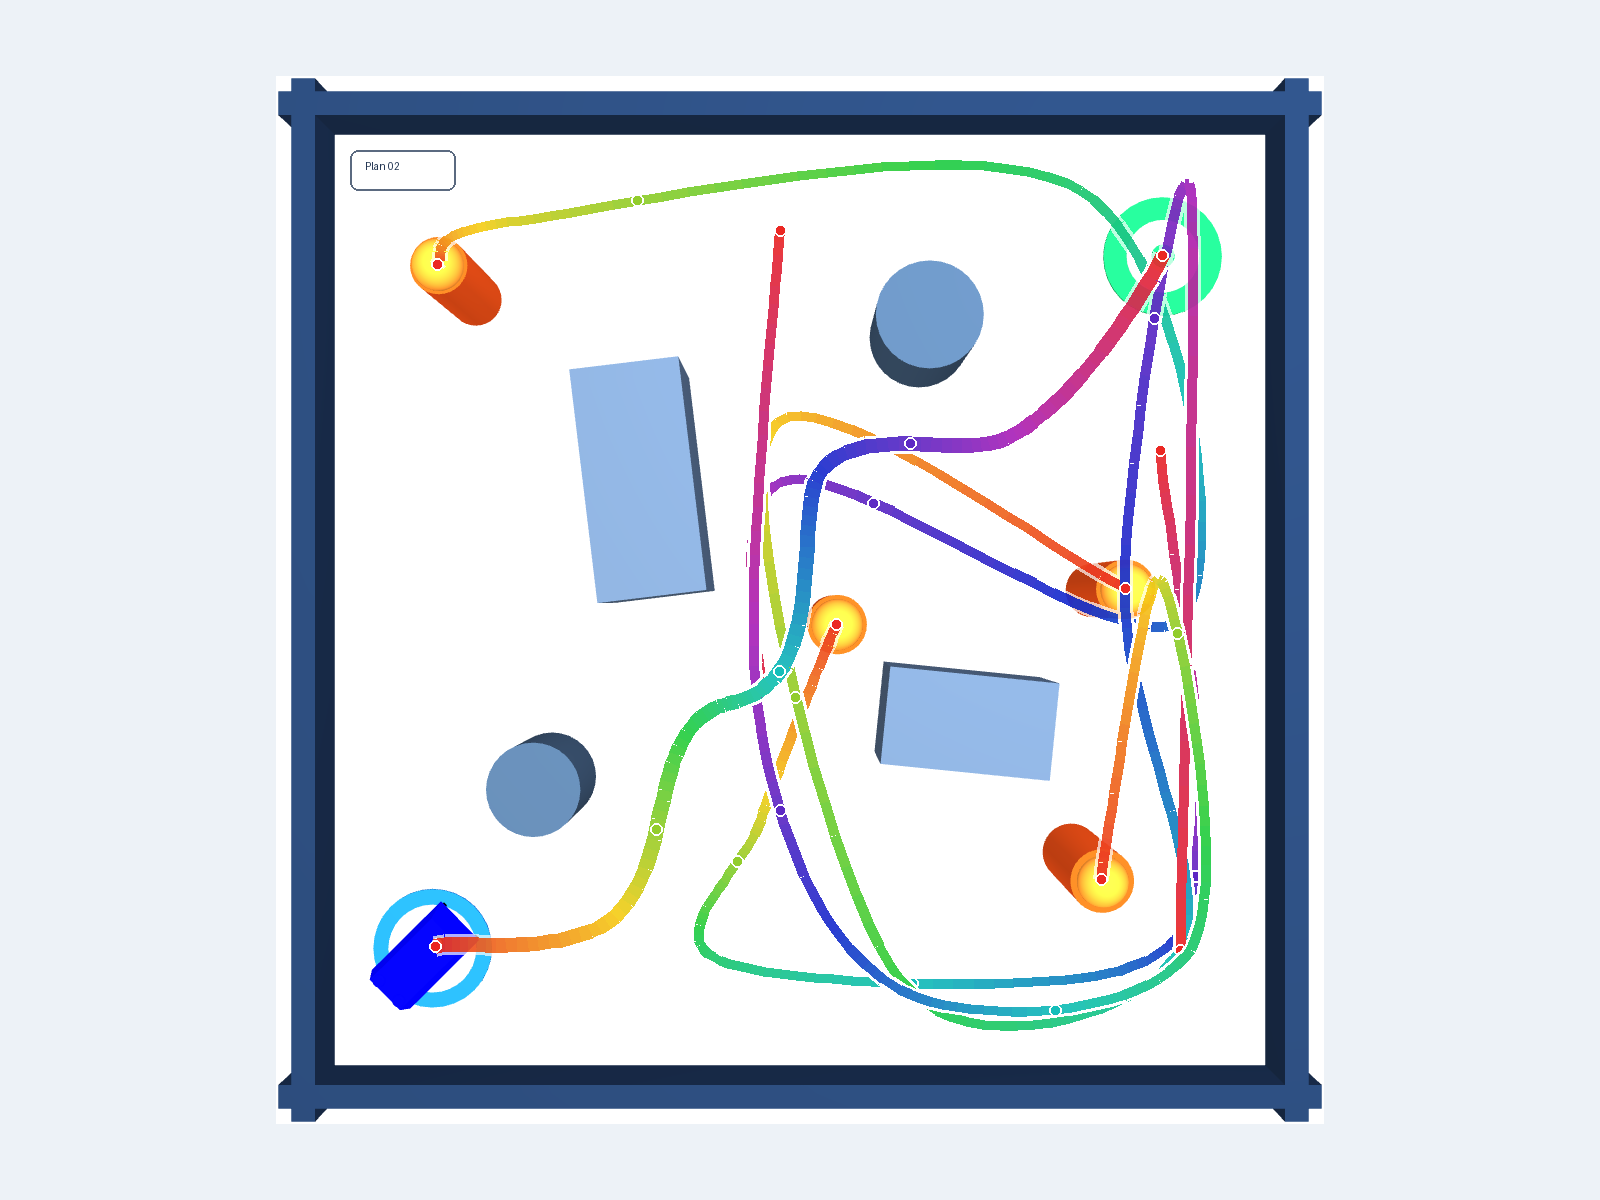
\includegraphics[width=\linewidth]{../rainbow_trajectory_synced_wavy_candidates_v3/rainbow_plan_02.png}
        \caption{Dense trajectory crossing (Plan 02)}
    \end{subfigure}\hfill
    \begin{subfigure}[t]{0.32\textwidth}
        \centering

        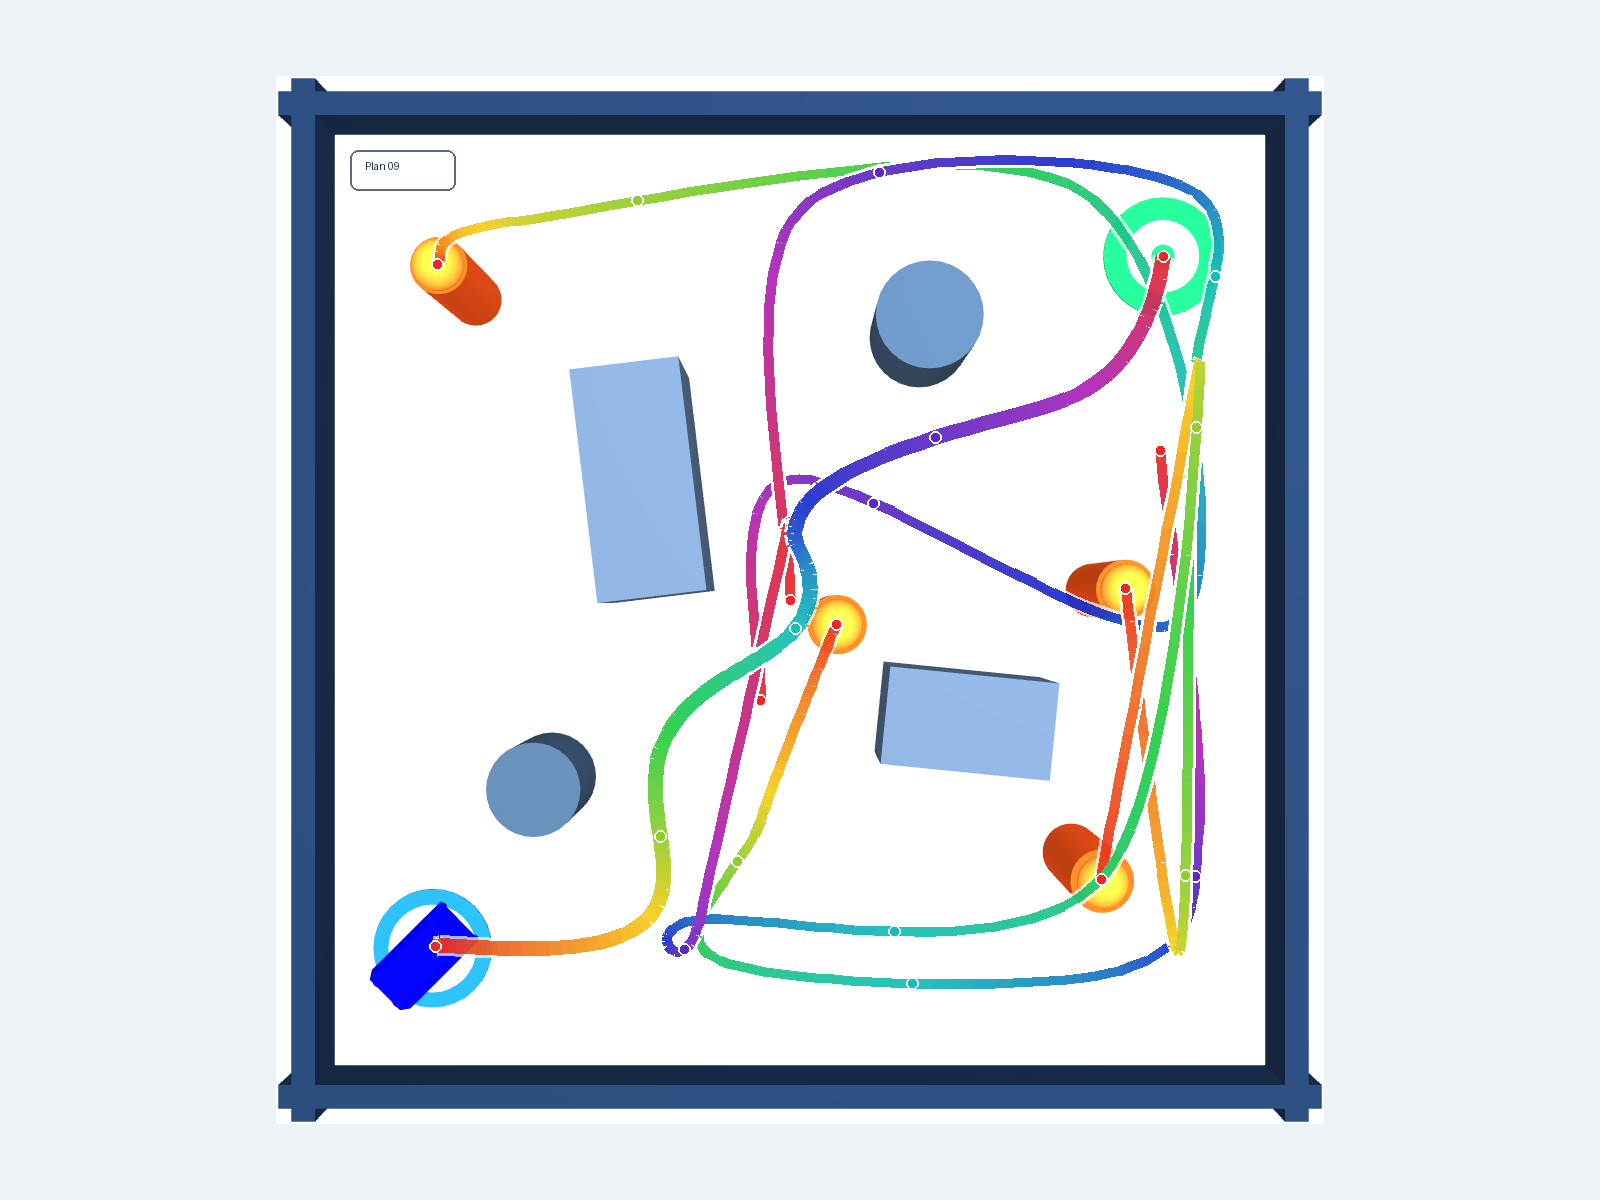
\includegraphics[width=\linewidth]{../rainbow_trajectory_synced_wavy_candidates_v3/rainbow_plan_09.png}
        \caption{Boundary detour (Plan 09)}
    \end{subfigure}\hfill
    \begin{subfigure}[t]{0.32\textwidth}
        \centering

        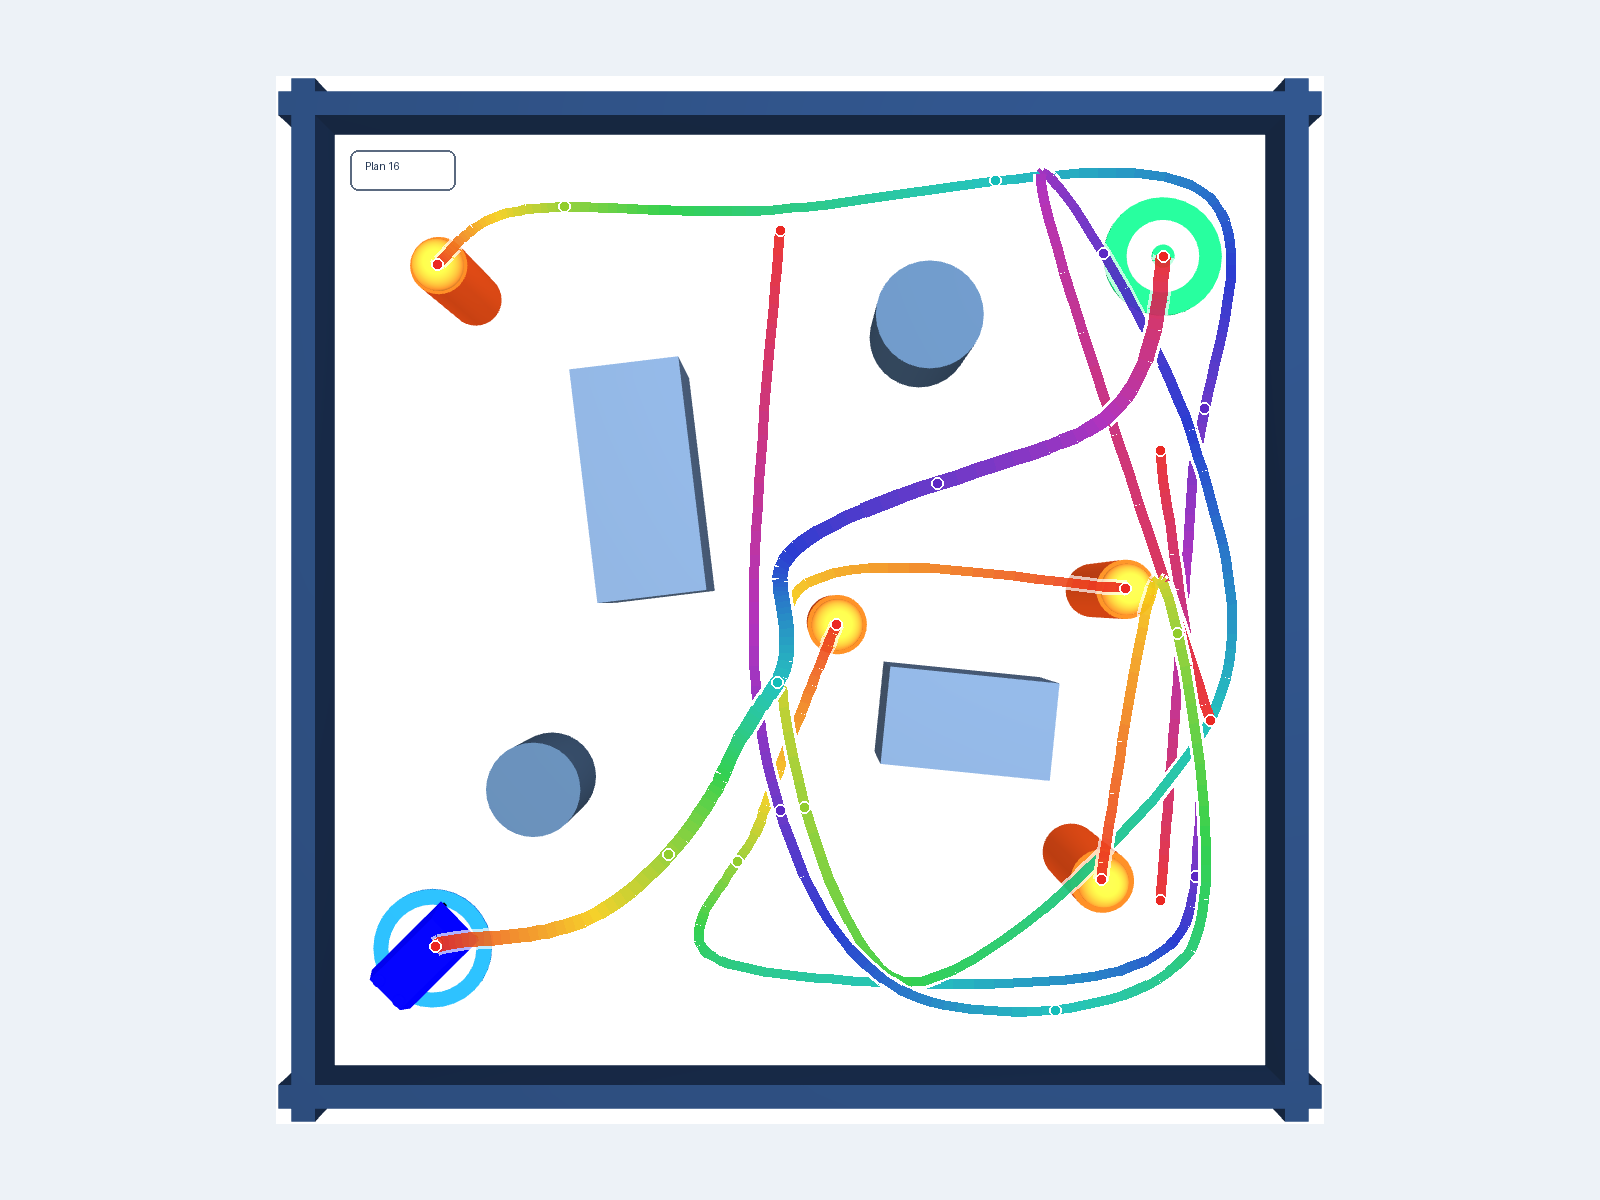
\includegraphics[width=\linewidth]{../rainbow_trajectory_synced_wavy_candidates_v3/rainbow_plan_16.png}
        \caption{Interaction with multiple dynamic obstacles (Plan 16)}
    \end{subfigure}
    \caption{Time-synchronised rainbow trajectories in the Gazebo dynamic scenario. The three panels use the same scene layout but correspond to different representative runs. Trajectory colour encodes simulation time, and sample points of the same colour denote the same instant; this synchronised representation can be used to judge whether the robot and the dynamic obstacles overlap in time at a spatial crossing.}
    \label{fig:gazebo_rainbow_trajectories}
\end{figure*}

The three trajectory groups show that the vehicle does not cross the scene along the geometrically shortest line from the lower-left to the upper-right corner; instead, it actively changes curvature and keeps spatial separation when approaching the central rectangular obstacle, the moving cylinder on the right, and the goal neighbourhood. In particular, where several trajectories cross geometrically, the corresponding sample points usually have different colours, which indicates that the robot and the obstacles avoid occupying the crossing region at the same time by staggering their arrival times. At the process level this shows that the policy can adjust its motion according to the dynamic occupancy relation, rather than merely following a fixed path on a static map. This figure provides qualitative evidence at the behavioural level only; the conclusions on task success rate, collision rate, and efficiency rest on the multi-seed IRSim results presented next.

\subsection{Quantitative Performance and Ablation}

Tables~\ref{tab:main_results} and~\ref{tab:efficiency_results} summarise the results over 5 random seeds and 50 episodes per method. All metrics take the within-seed mean as the statistical unit, and the cross-seed mean and standard error are reported. Figure~\ref{fig:paper_rates} compares the task-termination types, and Fig.~\ref{fig:paper_efficiency} compares the step count and path length.

\begin{table}[t]
    \centering

    \caption{Task-completion results of different navigation policies}
    \label{tab:main_results}
    \scriptsize

    \resizebox{\linewidth}{!}{\begin{tabular}{lccc}
\toprule
Method & Success rate $\uparrow$ & Collision rate $\downarrow$ & Timeout rate $\downarrow$ \\
\midrule
DRL-VO & 60.0 $\pm$ 3.2 & 36.0 $\pm$ 4.0 & 4.0 $\pm$ 2.4 \\
PVO & 64.0 $\pm$ 5.1 & 30.0 $\pm$ 6.3 & 6.0 $\pm$ 4.0 \\
AVO & 76.0 $\pm$ 6.8 & 10.0 $\pm$ 6.3 & 14.0 $\pm$ 5.1 \\
AVO-UQ & 60.0 $\pm$ 7.1 & 4.0 $\pm$ 2.4 & 36.0 $\pm$ 6.8 \\
\bottomrule
\end{tabular}
}
\end{table}

\begin{figure}[t]
    \centering

    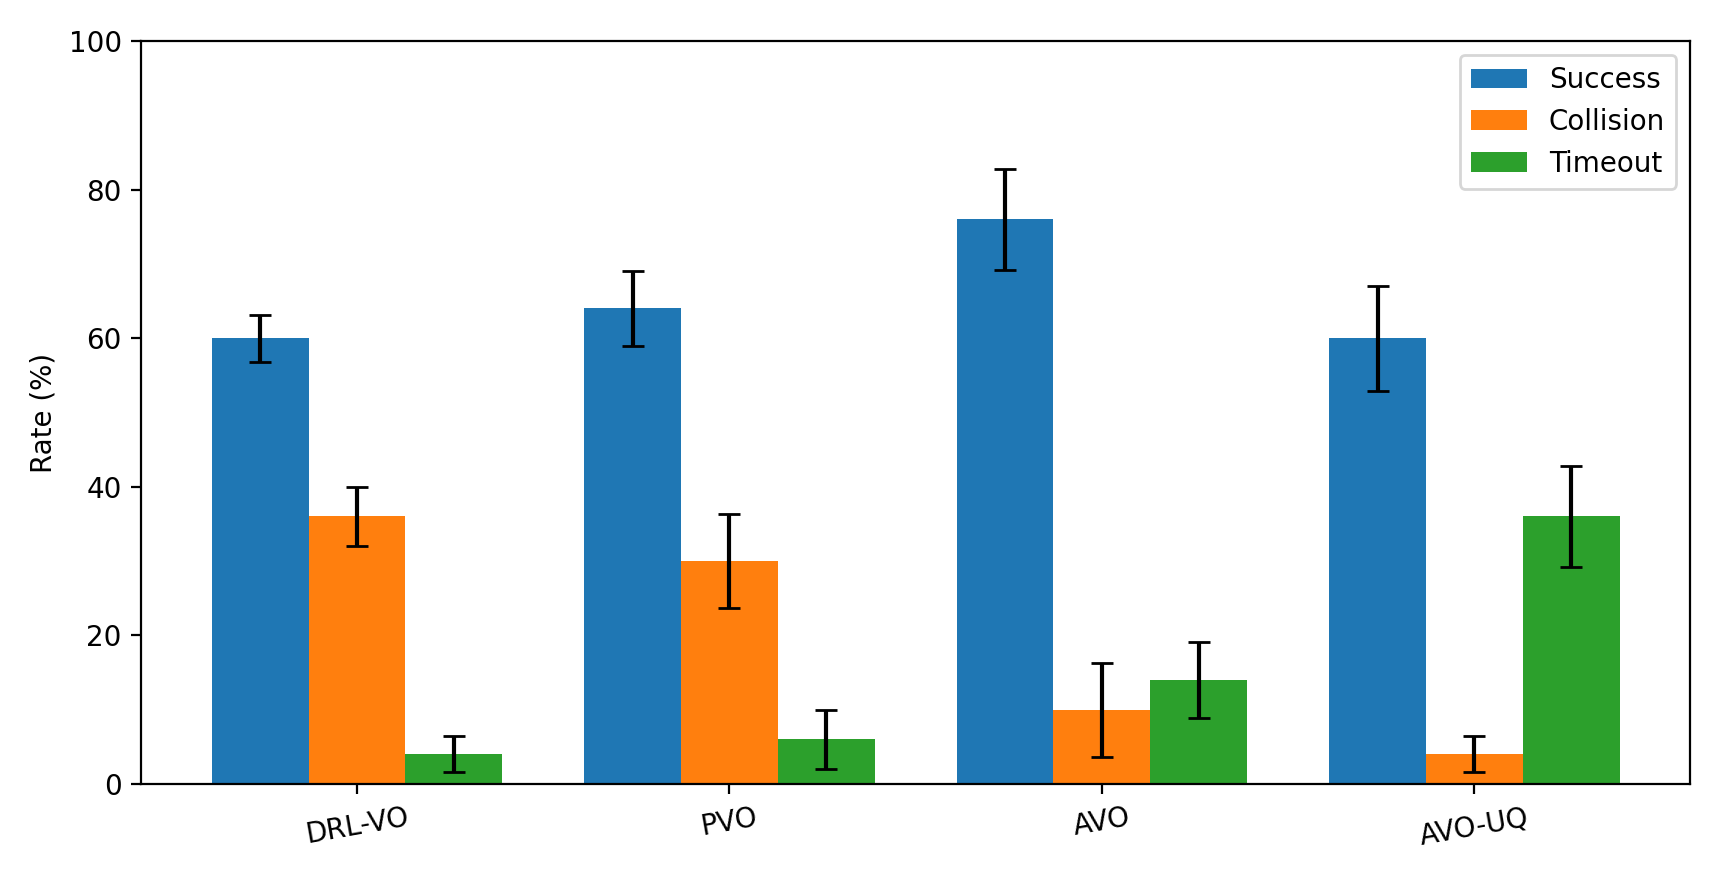
\includegraphics[width=0.85\linewidth]{../experiments/paper_results/paper_pvo_main_rates.png}
    \caption{Success rate, collision rate, and timeout rate over multiple random seeds. Error bars denote the per-seed standard error.}
    \label{fig:paper_rates}
\end{figure}

\begin{table}[t]
    \centering

    \caption{Efficiency and mode metrics of different navigation policies}
    \label{tab:efficiency_results}
    \scriptsize

    \resizebox{\linewidth}{!}{\begin{tabular}{lccccc}
\toprule
Method & Steps $\downarrow$ & Path $\downarrow$ & Switches $\downarrow$ & Lat./par. ratio & Time/ms $\downarrow$ \\
\midrule
DRL-VO & 41.80 $\pm$ 8.12 & 2.67 $\pm$ 0.14 & -- & -- & 0.58 $\pm$ 0.03 \\
PVO & 8.03 $\pm$ 1.25 & 1.25 $\pm$ 0.18 & 0.91 $\pm$ 0.06 & 88.5 $\pm$ 6.1 & 6.31 $\pm$ 0.40 \\
AVO & 96.34 $\pm$ 12.45 & 4.20 $\pm$ 0.41 & 14.55 $\pm$ 1.85 & 48.6 $\pm$ 7.2 & 7.40 $\pm$ 0.10 \\
AVO-UQ & 108.57 $\pm$ 7.62 & 3.02 $\pm$ 0.48 & 17.67 $\pm$ 1.74 & 37.0 $\pm$ 5.2 & 5.63 $\pm$ 0.58 \\
\bottomrule
\end{tabular}
}
\end{table}

In Table~\ref{tab:efficiency_results}, ``--'' indicates that the corresponding compared implementation did not record per-instant discrete motion-mode labels, and it is therefore not included in the statistics of mode switches and of the lateral/parallel ratio; this missing entry does not mean that the method uses a different robot chassis.

\begin{figure}[t]
    \centering

    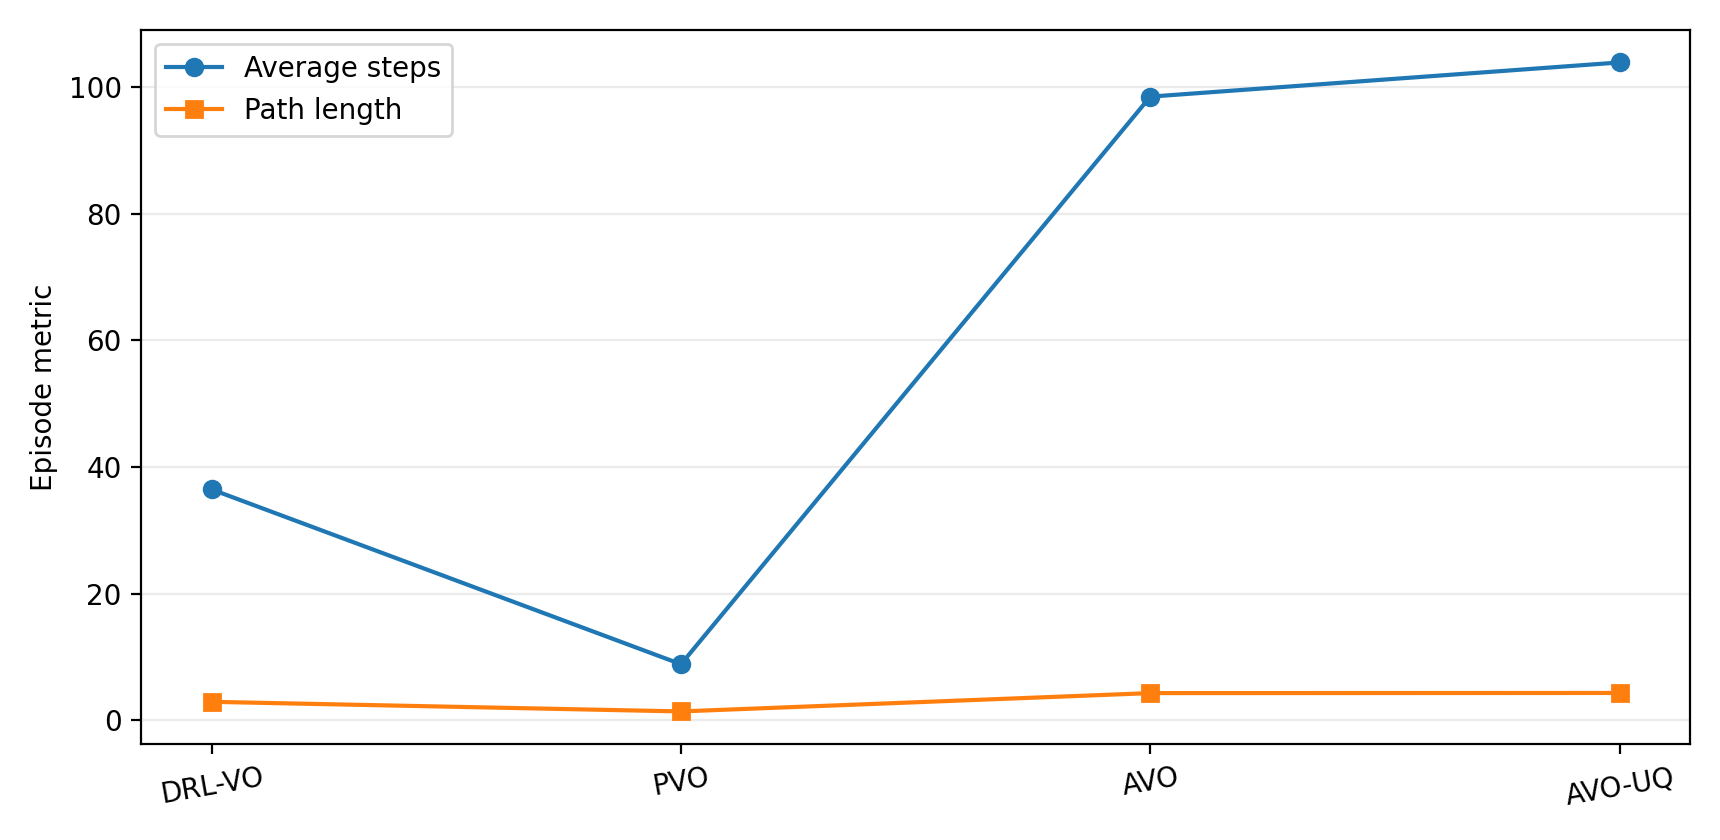
\includegraphics[width=0.85\linewidth]{../experiments/paper_results/paper_pvo_efficiency.png}
    \caption{Comparison of average steps and path length. AVO and its UQ extension trade longer detours, waiting, and risk interventions for a lower collision rate.}
    \label{fig:paper_efficiency}
\end{figure}

First, ordinary PVO attains a success rate of $64.0\%\pm5.1\%$, slightly above the $60.0\%\pm3.2\%$ of DRL-VO, while the collision rate drops from $36.0\%\pm4.0\%$ to $30.0\%\pm6.3\%$. Since both run on the 4WIS platform, this difference can no longer be explained by a change in chassis manoeuvrability; it reflects the limited benefit obtained when the current-frame collision judgement is extended from a deterministic VO to a probabilistic danger set. Ordinary PVO can absorb a certain amount of state and velocity estimation error, but it remains restricted by single-frame constant-velocity extrapolation and by a zero-latency prediction origin, so the reduction in collision rate is limited.

After adding action-conditioned future-risk filtering, the success rate of AVO rises to $76.0\%\pm6.8\%$ and the collision rate falls to $10.0\%\pm6.3\%$. Relative to ordinary PVO, the success rate improves by 12 percentage points and the collision rate drops by 20 percentage points, but the timeout rate also rises from $6.0\%$ to $14.0\%$. This baseline result shows that, in the present task, merely making the current-frame velocity obstacle probabilistic yields limited benefit, whereas the joint judgement of a candidate action and short-horizon future occupancy provides more effective action filtering. This result reflects the overall benefit of the action-conditioned risk module in the base scenario; the independent effects of history length, effective latency, and motion pattern are examined separately by the controlled experiments in Tables~\ref{tab:controlled_frequency}--\ref{tab:controlled_history}. The average step count and path length of AVO increase to $96.34\pm12.45$ and $4.20\pm0.41$, respectively, which shows that hard safety filtering trades longer detours and waiting for a reduction in collisions.

AVO-UQ reduces the collision rate further to $4.0\%\pm2.4\%$, but the success rate falls back to $60.0\%\pm7.1\%$, the timeout rate rises to $36.0\%\pm6.8\%$, and the average step count reaches $108.57\pm7.62$. The uncertainty penalty is therefore not a cost-free safety gain: in the absence of risk calibration and stall-recovery mechanisms, the additional conservatism converts part of the collisions into timeouts. What this ablation reveals is not a single ``best method'', but an explicitly adjustable three-way trade-off among risk tolerance, task-completion rate, and traversal efficiency.

\subsection{Control Frequency and Effective Reaction Window}

Table~\ref{tab:controlled_frequency} gives the control-frequency results at a fixed observation frequency of $50$~Hz. When the control frequency rises from $5$~Hz to $50$~Hz, the $T_{\mathrm{eff}}$ of AVO drops from $245$~ms to $65$~ms, its success rate rises from $58\%$ to $73\%$, and its collision rate falls from $22\%$ to $13\%$; the success rate of ordinary PVO rises from $50\%$ to $69\%$ and its collision rate falls from $30\%$ to $20\%$. This shows that shortening the action-update interval alone improves the reaction capability of all methods, so the entire benefit under high-frequency conditions should not be attributed to history modelling. At the same time, at $20$~Hz and $50$~Hz the success rate of AVO is $74\%$ and $73\%$ respectively, a difference that is already small, indicating diminishing marginal benefit at high frequency.

Within the same frequency sweep, AVO-UQ consistently maintains a lower collision rate---$10\%$ at $5$~Hz and $5\%$ at $50$~Hz---but its timeout rate is $40\%$ and $29\%$ respectively. The UQ branch therefore mainly enlarges the safety margin, without necessarily improving the task-completion rate. The per-step inference time in the table is about $0.65$--$7.47$~ms, which is below the $20$~ms period of a $50$~Hz control loop; in this experiment, the main variation in $T_{\mathrm{eff}}$ comes from the sampling and control-update interval rather than from the inference module itself.

\subsection{End-to-End Latency Robustness}

Table~\ref{tab:controlled_latency} fixes the control frequency at $20$~Hz and progressively adds $0$--$300$~ms of extra latency. As $T_{\mathrm{eff}}$ grows, the success rate of every method decreases and the collision rate increases, but action-conditioned future risk degrades more slowly. Taking $300$~ms as an example, AVO reaches a success rate of $55\%$ and a collision rate of $28\%$, which is 16 percentage points higher and 15 percentage points lower, respectively, than the $39\%$ and $43\%$ of ordinary PVO. The collision rate of AVO-UQ drops further to $18\%$, but its timeout rate reaches $36\%$, again demonstrating the efficiency cost of conservative filtering.

Latency also affects the calibratability of the risk score. The Brier score/ECE of ordinary PVO increases from $0.11/0.07$ to $0.21/0.14$, that of AVO from $0.08/0.040$ to $0.14/0.080$, and that of AVO-UQ from $0.060/0.030$ to $0.100/0.070$. This trend shows that history- and action-conditioned risk does not eliminate the prediction difficulty caused by latency, but can retain a relatively stable ranking capability under a longer effective reaction window; this is precisely the experimental meaning of moving the prediction origin from the current instant to the future window after the action takes effect.

\subsection{Obstacle Motion-Pattern Boundary}

Table~\ref{tab:controlled_motion} orders the results by the complexity of the future obstacle motion. Under constant-velocity motion the success rates of ordinary PVO and AVO are $74\%$ and $77\%$ and their collision rates are $15\%$ and $10\%$, a small gap that matches the condition in which the constant-velocity assumption is relatively appropriate. When the motion pattern changes to constant acceleration, smooth turning, stop-and-go, and sudden reversal, the success-rate difference of AVO over ordinary PVO widens successively to $9$, $11$, $15$, and $17$ percentage points, and the collision-rate difference widens to $11$, $11$, $13$, and $16$ percentage points. This sequence of results links the benefit of the method to the nonlinearity of obstacle motion, instead of claiming broadly that single-frame VO fails in all scenarios.

The partial-occlusion condition further amplifies the effect of insufficient state: the success rate of ordinary PVO drops to $40\%$ and its collision rate rises to $41\%$, whereas AVO still reaches a $58\%$ success rate and a $24\%$ collision rate. AVO-UQ obtains the lowest collision rate in all six patterns, but its timeout rate lies between $31\%$ and $40\%$, which shows that it is better suited as a safety-first configuration and should not be evaluated by success rate alone.

\subsection{Historical State and State-Quality Ablation}

Table~\ref{tab:controlled_history} further compares history length, effective latency, and state source within a single set of conditions. Under the current-frame condition, AVO reaches a success rate of $68\%$ and a collision rate of $20\%$, close to the $67\%$ and $21\%$ of single-frame PVO; when the history window grows from $K=1$ to $K=3$ and $K=5$, the success rate of AVO rises to $72\%$ and $75\%$ and its collision rate falls to $15\%$ and $11\%$. At the same time, AUROC increases from $0.70$ to $0.77$ and $0.83$, and ECE decreases from $0.08$ to $0.07$ and $0.05$, reflecting an improvement in both risk-ranking ability and probabilistic calibration.

After adding $50$~ms of extra latency, the success rate at $K=5$ falls back to $70\%$ and the collision rate rises to $15\%$, which shows that historical information provides compensation but is not sufficient to offset a longer effective reaction window completely. Under the oracle state reference, AVO with $K=5$ reaches a $78\%$ success rate, a $9\%$ collision rate, $0.90$ AUROC, and $0.03$ ECE; a gap remains relative to the $K=5$ condition with estimated states, which indicates that perception state quality is a key factor for risk prediction. The AUROC/ECE in Table~9 quantify the discriminative ability and the probabilistic calibration ability of the historical risk head; DRL-VO does not output a probability, so the corresponding calibration metrics are recorded as N/A.

\section{Discussion}

The results above form a two-level chain of evidence, from ``baseline benefit'' to ``applicability boundary''. On the same 4WIS platform, ordinary PVO achieves only a limited improvement over DRL-VO, whereas AVO reduces the collision rate and raises the success rate relative to ordinary PVO at the same time, which shows that candidate-action conditioning plus short-horizon future-occupancy rollout is more effective than merely making the current-frame risk probabilistic. The control-frequency experiment further shows that high-frequency rolling updates by themselves improve the reaction capability of all methods; the latency and motion-pattern experiments show that the relative advantage of AVO becomes more pronounced when the effective reaction window grows longer or when obstacle motion deviates from constant velocity. The central claim of this paper should therefore be stated as a conditional proposition: the value of history and future-risk modelling depends on whether the state covers the critical interval around the moment at which the action takes effect.

The results for AVO-UQ reveal another important trade-off. It usually attains the lowest collision rate in the frequency sweep, the latency sweep, and the motion-pattern sweep, but its timeout rate remains consistently high, which shows that the conservative risk correction converts part of the collision risk into waiting, detours, and task timeouts. A practical system should therefore not optimise the collision rate alone, but should jointly consider the success rate, collision rate, timeout rate, minimum safety distance, path length, and intervention frequency, and select the risk threshold according to the application scenario.

Tables 6--9 report the actual controlled-experiment results, where the AUROC and ECE in Table~9 come from the state ablation and probabilistic calibration procedure of the historical risk head; the base main experiment and Tables 6--8 use the action-conditioned geometric surrogate as the quantitative risk implementation. Every controlled condition uses $N=200$ episodes, the tables give condition-level point estimates, and together with the cross-seed statistics of the baseline experiments they characterise the safety, efficiency, and applicability boundary of the method.

In addition, the quantitative 4WIS simulation adopts idealised planar kinematics and does not explicitly model wheel-level steering constraints, maximum steering-rate limits, or actuator dynamics; the Gazebo trajectories mainly serve to display process-level behaviour. The conclusions of this paper therefore hold for a unified 4WIS kinematic platform, for the given perception conditions, and for the reported effective reaction window.

\section{Conclusion}

This paper restricts the problem to the following question: when the environment is partially observable and the effective reaction window is non-negligible, is the current state sufficient to support the safety judgement of multimodal 4WIS candidate actions? To this end, AVO represents the collision risk as a joint function of the observation history, the candidate action, and the future execution window, and embeds risk assessment into the safety filtering performed before action execution. The four methods are compared on the same 4WIS platform; in the base multi-seed results, AVO raises the success rate from $64.0\%\pm5.1\%$ to $76.0\%\pm6.8\%$ and reduces the collision rate from $30.0\%\pm6.3\%$ to $10.0\%\pm6.3\%$ relative to ordinary PVO, while AVO-UQ reduces the collision rate further to $4.0\%\pm2.4\%$ at the cost of a timeout rate rising to $36.0\%\pm6.8\%$.

The controlled experiments in Tables 6--9 unfold this conclusion into four testable dimensions: the control frequency determines the length of the effective reaction window, the end-to-end latency determines the misalignment between the current observation and the moment at which the action takes effect, the obstacle motion pattern determines how applicable constant-velocity extrapolation is, and the history window and state source determine how much dynamic information risk prediction can recover. The results exhibit a clear boundary trend: under high frequency, low latency, and constant velocity the differences between methods shrink; once latency increases, or turning or partial occlusion appears, the advantage of action-conditioned future risk widens; and the uncertainty correction exchanges a higher timeout rate for a lower collision rate.

\bibliographystyle{ieeetr}
\bibliography{references}

\end{document}
